
\section{The sequential algorithm: Color Coding}
\label{sec:sequential}


\begin{table}[hptb]
\caption{Notations}
\label{tab:notations}
\centering{
\begin{tabular}{c|c|c|c}
\hline
symbol & description & symbol & description \\
\hline
$G$ & graph & $T, T', T''$ & template and sub-templates \\
$n, m$ & \# nodes, \# edges & $k$ & \# nodes in $T$ \\
$\rho$ & root of $T$ & $S, s_i$ & color set, the $i^{th}$ color \\
$d(v)$ & degree of node $v$ & $N(v)$ & neighbors of node $v$ \\
\hline
\end{tabular}
}
\end{table}



%\subsection{Color Coding for Subgraph Counting}
%\label{subsec:intro-color-coding}

We briefly introduce the color coding algorithm for subgraph
counting~\cite{alon1995color}, which gives a randomized approximation scheme for
counting trees in a graph.  Some of the notation used in the paper is listed in
Table~\ref{tab:notations}.

\noindent
\textbf{High level description.}
There are two main ideas underlying the color coding algorithm of~\cite{alon1995color}.
\begin{enumerate}[leftmargin=4mm, noitemsep, topsep=0pt]
\item
\textbf{Colorful embeddings}:

Color the nodes of the graph with $k$ colors where $k \geq |V_T|$, and only count
``colorful'' embeddings---an embedding $H$ of the template $T$ is colorful if
each node in $H$ has a distinct color.  The advantage of this is that the number
of colorful embeddings can be counted by a simple and natural dynamic program.

\begin{enumerate}
\item
In particular, let $C(v, T(\rho), S)$ be the number of colorful embeddings of $T$ with node
$v \in V_G$ mapped to the root $\rho$, and using the color set $S$, where
$|V_{T}| = |S|$. 
\item
Suppose $(\rho=u_1, u_2)$ is an edge incident on the root node
$\rho$ in $T$. Let tree $T$ be partitioned into trees $T_1$ and $T_2$ when the
edge $(u_1, u_2)$ is removed, with roots $\rho_1=u_1$ and $\rho_2=u_2$ of the
trees $T_1$ and $T_2$, respectively.
\item
Suppose $S_1$ and $S_2$ are disjoint subsets of colors
such that $|S_1|=|V_{T_1}|$, $|S_2| = |V_{T_2}|$. Let $H_1$ and $H_2$ be two
colorful embeddings of $T_1$ and $T_2$ using color sets $S_1$ and $S_2$, respectively,
with $\rho_1$ and $\rho_2$ mapped to neighboring nodes $v_1\in V_G$ and
$v_2\in V_G$, respectively. Then, $H_1$ and $H_2$ must be \emph{non-overlapping},
because they have distinct colors.
\item
Therefore, 
\begin{align*}
C(v_1, T, S) & = \sum_{v_2\in N(v_1)} \sum_{S=S_1\cup S_2} C(v_1, T_1(v_1), S_1) \cdot\\
& \qquad \qquad \qquad \qquad  \qquad C(v_2, T_2(v_2), S_2),
\end{align*}
where the first summation is over all neighbors $v_2$ of $v_1$ and the
second summation is over all partitions $S_1\cup S_2$ of $S$.
\end{enumerate}
\item
\textbf{Random colorings}:
If the coloring is done randomly with $k=|V_T|$ colors, there is a reasonable
probability $\frac{k!}{k^k}$ that an embedding is colorful---this allows us to
get a good approximation to the number of embeddings.
\end{enumerate}

%Figure~\ref{fig:paths} shows an example of the quantities
%$C(v, T_i(\rho_i), S_i)$, and a recurrence relation for computing them, using
%the counts corresponding to smaller trees.  The complete algorithm (described
%below) involves (i) partitioning the template into sub-templates, and (ii) a
%dynamic program to compute the colorful counts.

\begin{algorithm}[ht]
  \caption{The sequential color coding algorithm.}
  \label{alg:sequential}
  \begin{algorithmic}[1]
\STATE \textbf{Input:} Graph $G=(V, E)$ and template $T=(V_T, E_T)$
\STATE \textbf{Output:} Approximation to $emb(T, G)$
\STATE
\STATE For each $v\in V_G$, pick a color $c(v)\in S=\{1,\ldots,k\}$ uniformly at random,
where $k=|V_T|$.

\STATE Partition the tree $T$ into subtrees recursively to form a set $\mathcal{T}$
using algorithm \textsc{Partition}$(T(\rho))$. For each tree $T'\in\mathcal{T}$,
we have a root $\rho'$. Further, if $|V_{T'}|>1$, $T'$ is partitioned into
two trees $T'_1, T'_2$ with roots $\rho'_1=\rho'$ and $\rho'_2$, respectively,
which are referred to as the active and passive children of $T'$.

\STATE For each $v\in V_G$, $T_i\in\mathcal{T}$ with root $\rho_i$, and subset $S_i\subseteq S$,
with $|S_i|=|T_i|$, we compute $C(v, T_i(\rho_i), S_i)$ using the the recurrence
(~\ref{eq:color-coding-dp}) below:

\begin{equation}
\label{eq:color-coding-dp}
\begin{array}{lcl}
\hspace*{-0.2in}c(v, T_i(\rho_i), S_i) = \frac{1}{d}\displaystyle\sum\limits_{u}
\displaystyle\sum c(v, T_i'(\rho_i), S_i') \cdot\\
\hspace*{1.4in}c(u, T_i''(\tau_i), S_i''),
\end{array}
\end{equation}

where $d$ is equal to one plus the number of siblings of
$\tau_i$ which are roots of subtrees isomorphic to $T_i''(\tau_i)$.

\STATE For the $j$th random coloring, let
\begin{equation}
\label{eq:color-coding-sum}
\begin{array}{lcl}
C^{(j)} = \frac{1}{q}\frac{k!}{k^k}\sum_{ v \in V_G} c(v, T(\rho), S),
\end{array}
\end{equation}
where $q$ denotes the number of node $\rho' \in
V_T$ such that $T$ is isomorphic to itself when $\rho$ is mapped to $\rho'$.

\STATE
Repeat the above steps $N=O(\frac{e^k\log(1/\delta)}{\varepsilon^2})$ times,
and partition $N$ estimates $C^{(1)},...,C^{(N)}$ into $t=O(\log(1/\delta))$ sets. Let
$Z_j$ be the average of set $j$. Output the median of $Z_1,...,Z_t$.
  \end{algorithmic}
\end{algorithm}



\begin{algorithm}[ht]
 \caption{\emph{Partition($T(\rho)$)}}
 \label{alg:partition}
\begin{algorithmic}[1]
 \IF{$T \notin \mathcal{T}$}
  \IF{$|V_T| = 1$}
    \STATE $\mathcal{T} \leftarrow T$
  \ELSE
   \STATE Add $T$ to $\mathcal{T}$
   \STATE Pick $\tau \in N(\rho)$, the set of the neighbors of $\rho$,
and partition $T$ into two sub-templates by cutting the edge $(\rho, \tau)$

   \STATE Let $T'$ be the sub-template containing $\rho$ (name as \textit{active child}) and
$T''$ the other (name as \textit{passive child})

   \STATE Partition($T'(\rho)$)
   \STATE Partition($T''(\tau)$)
  \ENDIF
 \ENDIF
\end{algorithmic}
\end{algorithm}


%The sequential color coding algorithm is proposed first in~\cite{alon1995color}
%by Alon \emph{et al.} in 1995. It is a randomized approximation algorithm which
%converges with running time
%$O(m|E|2^me^m\log{(1/\delta)}\frac{1}{\varepsilon^2})$, where $\varepsilon$ and
%$\delta$ are error and confidence parameters, respectively. It consists of the
%following three steps:
%
%\begin{enumerate}
%
%\item Randomly color the nodes in graph $G$ with a color set $S$ which contains $m$
%colors, where $m = |V_T|$, 
%
%\item Using dynamic programming, compute the number of ``colorful''
%embeddings of template $T$, denoted as $c$. A subgraph is colorful if each of
%its node has distinct color.  The dynamic programming is represented by Eq.
%~\ref{eq:color-coding-dp}.
%
%\begin{equation}
%\label{eq:color-coding-dp}
%\begin{array}{lcl}
%
%\hspace*{-0.2in}c(v, T_i(\rho_i), S_i) = \frac{1}{d}\displaystyle\sum\limits_{u}
%\displaystyle\sum c(v, T_i'(\rho_i), S_i') \cdot\\
%\hspace*{1.4in}c(u, T_i''(\tau_i), S_i'')
%
%\end{array}
%\end{equation}
%
%Here, the notation $c(v, T_i(\rho_i), S_i)$ represents the number of the colorful
%subgraphs in $G$ that are isomorphic to $T_i$ (rooted at $\rho$) with $\rho$
%mapped to $v \in G$, and each embedding is colored with $S_i$. The first
%summation is over all $u \in neighbor(v)$ and the second summation is over all $S_i',
%S_i''$ such that $S_i' \cap S_i'' = \emptyset, S_i' \cup S_i'' = S_i$. Here $d$
%is the over-counting factor and is equal to one plus the number of siblings of
%$\tau_i$ which are roots of subtrees isomorphic to $T_i''(\tau_i)$.
%
%\item After dynamic programming, we have $c(v, T(\rho), S)$ for all $v \in
%V_G$. Then we can compute the total number of colorful embeddings with Eq.
%~\ref{eq:color-coding-sum}.
%
%\begin{equation}
%\label{eq:color-coding-sum}
%\begin{array}{lcl}
%C = \frac{1}{q}\sum_{\forall v \in V_G} c(v, T(\rho), S)
%\end{array}
%\end{equation}
%
%Here $q$ is another over counting factor, i.e., the number of node $\rho' \in
%V_T$ such that $T$ is isomorphic to itself when $\rho$ is mapped to $\rho'$.
%
%
%\item Suppose the number of all embeddings of $T$ is $Y$, then it is easy to
%obtain $C = Y \cdot \frac{m!}{m^m}$, therefore, we can compute $Y = C \cdot
%\frac{m^m}{m!}$. 
%
%\end{enumerate}

Algorithm~\ref{alg:sequential} describes the sequential color coding algorithm.
Figure~\ref{fig:example-dp} gives an example of computing Eq. 1.

\begin{figure}[htbp]
\centerline{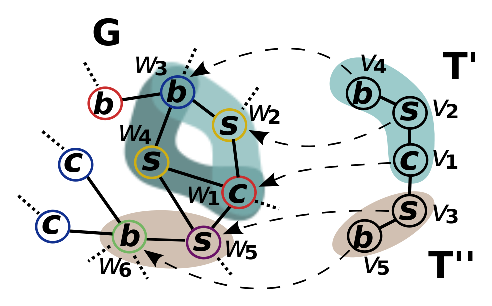
\includegraphics[width=0.24\textwidth]{plots/paths.eps}}

\caption{The example shows one step of the dynamic programming in color coding.
$T$ in Figure~\ref{fig:isomorphism} is split into $T'$ and $T''$. To count
$C(w_1, T(v_1), S)$, or the number of embeddings of $T(v_1)$ rooted at $w_1$,
using color set $S=\{\underline{r}ed, \underline{y}ellow, \underline{b}lue,
\underline{p}urple, \underline{g}reen\}$, we first obtain $C(w_1, T'(v_1), \{r,
y, b\})=2$ and $C(w_5, T''(v_3), \{p, g\})=1$.  Then, $C(w_1, T(v_1), S) =
C(w_1, T'(v_1), \{r, y, b\}) C(w_5, T''(v_3), \{p, g\})=2$.  The
embeddings of $T$ are subgraphs with nodes $\{w_3, w_4, w_1, w_5, w_6\}$ and
$\{w_3, w_2, w_1, w_5, w_6\}$. Here $s, c, b$ represents the label of the nodes.
Details of labeled subgraph counting can be found at~\cite{zhao2012sahad}.}

\label{fig:example-dp}
\end{figure}

